\documentclass{ltjbook}
\usepackage{docmute} 
\usepackage{../../myStyle} 

\begin{document}
\chapter{実験計画法の基礎とRCT}
\label{ch17_RCT}

前回，統計的な検定で2群の平均値の差を判定することを見てきました。
統計的な検定は，推定に基づいた「判断」であり，「意思決定」のための方法でもあったわけです。この方法を応用して，2群だけでなく3群以上の場合でも，差があるのかどうかを判定することを考えます。そのためには，差があるかどうかを見極めるための計画が重要になってきます。

この実験計画法＋統計的な検定は，心理学研究のスタンダードな方法の一つです。
ここからは心理学における実験と，その分析方法についての話に進んでいきます。


\section{ランダム化の意義と方法}
\label{RCT}
心理学は人間を対象にした学問であり，研究の方法はさまざまなものがあります。一般的には，調査，観察，実験，面接などの方法がとられます。ここでいう実験とは，皆さんが小中学校の理科の時間に習ったような実験と，同じようなものだと思っていただいて構いません。ただしその対象が人間になっているというところに，注意が必要なだけです。その注意というのは，もちろん倫理的な問題も多く含みますが，それに加えて，物理学の実験と違って研究の対象が意思を持っているというところです。そうした研究対象特有の問題に考慮しつつ，実験とはどのように進めていくべきかを考えてみましょう。

簡単なところから，小学校の理科でやるような実験として，次のような例を考えてみましょう。植物の種をまいて，植物の成長にはどういった要因が必要なのかを考える授業をするとします。ここでいろいろな条件を考えて実験を計画しますね。たとえば日向と日陰を比べればどちらが成長が速いのかとか，水をあげた場合とあげない場合とではどちらが成長が速いのかとか，どういった肥料をどれぐらいあげれば成長が速くなるのかといったことを検証したいとします。

たとえば日光の効果を検証したいのであれば，半分は日向に残りの半分は日陰に種をまいて，どちらの方が成長が良いかを記録するという方法で実験することになると思います。当然のことながらこの時重要になってくるのは，日向か日陰かという条件以外の要素を変更しないことです。たとえば日向にまいた種だけに水を与えるとか肥料を与えるといったことをすると，最終的に得られた成長の違いが日光によるものなのか，それ以外の要因によるものなのか区別できません。これでは研究の目的が果たせないわけです。実験をする場合は，検証したい条件の違い以外は均一にしておくということが必須です\footnote{このように介入が入り混じっていて効果が特定できなくなることを，要因が\keyterm{交絡}{こうらく}{confounding}するといいます。交絡という言葉は，字義通り「交わり，からまっている」という意味で，本当に見たい因果関係を切り出せないことを指します。}。

何を当たり前のことをと思われるかもしれませんが，人間の場合はさまざまな要因が絡み合っているので，何か1つの効果を見るために他のものを統制しようとしても，統制すべき要因が無数に考えられてしまうので，おのずと限界があるわけです。

人間を研究の対象にする場合の問題は他にもあります。まずこの授業でも冒頭のほうにお話ししたと思いますが，何を結果変数にするかというところも明確ではありません。人の気持ちのようなものが従属変数になっていたとして，その気持ちをどのように測定するのかという測定方法にもさまざまな注意すべき点があるでしょう。測定するべき対象が明確になっていたとしても，被験者に負担をかけすぎないかどうかは倫理的に検証されるべきです。また，研究対象が人間ですから，人間の回答は嘘をつかれることもあれば，間違うこともあれば，実験者の意図を汲んで自然な状態でない反応をすることもあります。こうした問題に対しては，\keyterm{二重盲検法}{にじゅうもうけんほう}{double blind experiment}を始めさまざまな方法で問題を回避しなければならないといった事は，心理学研究法の方で話を聞いていることと思います。

先に述べた測定の問題と，後半で述べた倫理的な問題を始めとする研究法の問題は横に置いたとしても，実験にはコントロールしてもコントロールしきれないものが含まれる事はお分かりいただけると思います。このコントロールしきれない部分のことを\keytermL{偶然誤差}{ぐうぜんごさ}と言いますが，偶然誤差に振り回されるだけではなくこれを積極的に利用することによって，実験の質を高めるために利用できます。偶然をハンドリングするのです！

人間を対象にした実験の例を考えてみましょう。たとえば新しく商品開発された3つのミネラルウォーターがあったとして，いろんな人に試し飲みしてもらって採点してもらったとします。このドリンクA,B,C について評価してもらうとして，その場合に気にしないといけないことがあります。1つはどの順番で飲んでもらうかということです。たとえばドリンクAに甘い味がついていたとして，その後でB,Cを飲むと味が薄いと評価されるかもしれません。あるいは1種類目$\to$2種類目$\to$3種類目と順番に飲んでいたとして，最後のほうはもうお腹がタポタポで全然味の評価ができないということがあるかもしれません。このようにどういう順番で飲むかとか，どの並びで飲むかといったことも評価に影響してきます。こうなってくるとこれはもう統制できませんので，諦めるのではなくて，逆に偶然の力を借りるのです。つまり，サイコロを振って1か2が出ればA，3か4が出ればBをまず飲む，といったようにし，人によって飲む順番も並びもバラバラになってしまえば，飲む順番や並びの効果があったとしても，相互に影響を殺しあって，平均をとればそれぞれのミネラルウォーターの評価として使うことができると考えるわけです。

ここでこのようにバラバラにするということを，言い方を変えると\keyterm{ランダム化}{らんだむか}{randomize}するといいます。英語でランダムrandomは確率とも訳されます\footnote{確率的に決まる変数のことを確率変数と言いますが，確率変数は英語でrandom variablesです。}。確率化すると言い換えても構いません。偶然をハンドリングするために，確率の力を借りようというわけです。

第\ref{ch10_probability}講で\keytermL{正規分布}{せいきぶんぷ}の話をしました。正規分布はさまざまな要因の積み重ねとして，つまり二項分布の極限の形で出てくる分布だということでした。この話をここで思い出してみましょう。人にはさまざまな個性があり，それを統制した上で実験をするなんて事は不可能です。しかし1人ではなくて多くの人間を集めてくると，ある変数については正規分布の形に近づいてくるでしょう。たとえば身長や体重といった生理的な指標や，学力や心理的な変数なども正規分布にしたがうと考えられるわけです。このときの正規分布の平均は，集団の代表的な値，真ん中あたりの人ということになるでしょう。偶然誤差の部分は平均がゼロになっていますから\footnote{プラスの要因とマイナスの要因，大きさもさまざまなので，それらが相殺し合う＝キャンセルアウトされる，といいます。}，系統的な特徴が平均のところに現れていると考えられるわけです。

このように，被験者一人一人の特徴はあるとしても，平均を取れば何らかの傾向があるはずです。誰が飲んでも美味しい飲み物とか，その逆ということはあるわけです。平均を取ることで，個性をキャンセルアウトしようということですね。
その上で，振り分けにも確率の力をかりてランダム化します。サイコロの目が偶数なら群A，奇数なら群B，というように無作為に群分けするのです。無作為にグループを分けていますから，どちらのグループにもさまざまな人が入ることになります。味覚に敏感な人やそうでない人など，今回の実験に関わる個性があったとしても，2つのグループの平均は，個性がキャンセルアウトされていますから，平均的には同程度の群が2つできたことになります。

心理学における実験で因果的な効果を考える場合は，無作為\footnote{無作為の反対，作為とは意図を持ったという意味です。無作為はその否定で，何の意図も持たずに，という意味です。}に群分けをし，一方を\keyterm{統制群}{とうせいぐん}{control group}，他方を\keyterm{実験群}{じっけんぐん}{experimental group}と呼びます。実験群には何らかの操作が加えられます。これに対して統制群には何もしない，あるいは何の効果もない同程度の介入をします\footnote{何もしないことが逆に何らかの意味や効果を持ってしまう可能性があるからです。人間を対象にした研究はややこしい！}。無作為に群分けしているので実験群のグループに含まれるさまざまな原因の効果は，統制群にも同程度に含まれているはずです。それが課題に影響を与えるものであったとしても，これは両群に同程度の効果を持っているはずです。介入の後で両群に何らかの心理学的な課題をさせるとか，反応を見るとかします。その結果のところで平均的な成績の差を比較します。何らかの要因があって，それが課題の成績にプラスに出るかマイナスに出るかといったことがあるかも知れませんが，群全体としてはそれは同程度のはずです。それを超えて群の間に差があるとしたら，その原因は操作をしたかしなかったかにあると言えるではありませんか。このように平均化することで，因果的な効果を考えることができるようになるのです(図\ref{fig:17_01})。この効果のことをとくに\keytermL{平均因果効果}{へいきんいんがこうか}と言います。

\begin{figure}[ht]
	\centering
	\caption{RCTの基本的枠組み}
	\label{fig:17_01}
	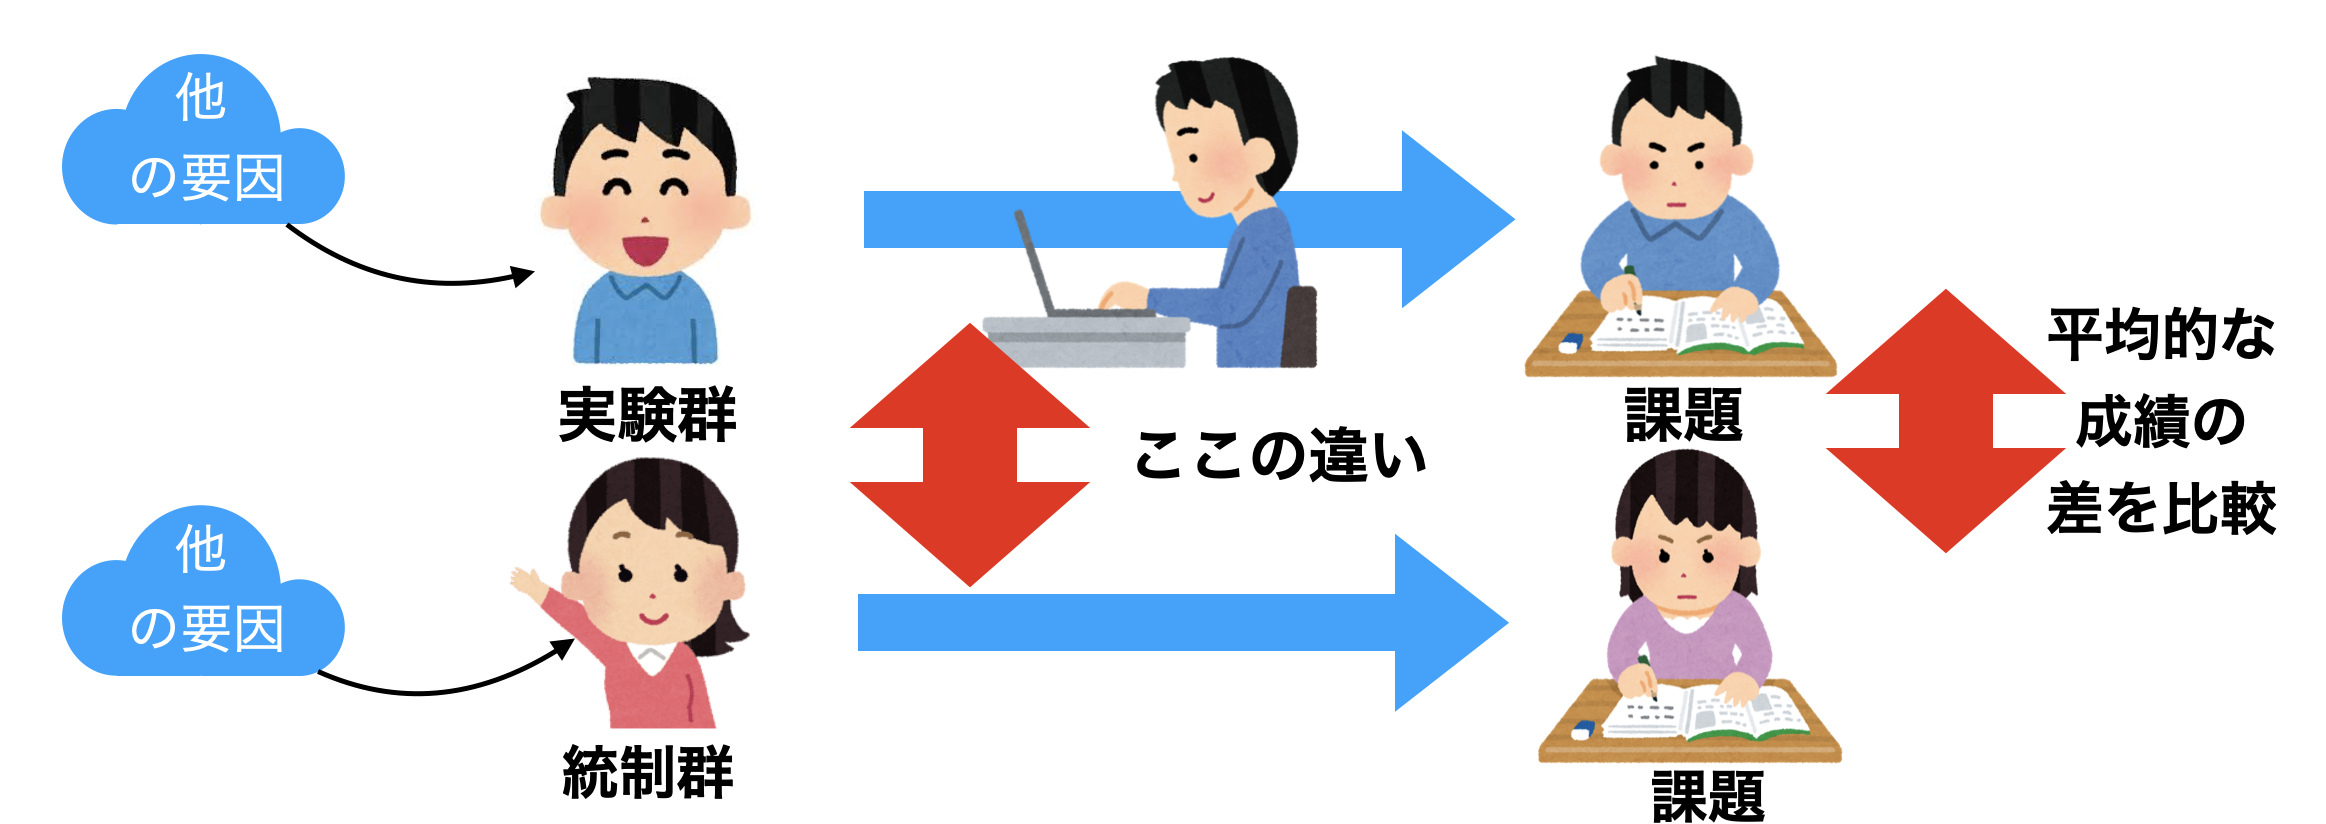
\includegraphics[keepaspectratio,width=0.8\linewidth]{figures/17_RCT/RCT.png}
\end{figure}

これが実験の基本的な枠組みです。集団の平均的な違いは，無作為に群分けすることで個体差を相互に打ち消し合うための仕掛けです。誤差をコントロールする方法の1つと言えるでしょう。この方法を\keyterm{ランダム化比較試験}{らんだむかひかくしけん}{randomized controlled trial; RCT}といいます。偶然誤差，あるいは個体差が相互に打ち消し合うのは，それらが正規分布に従うという特徴を生かした方法だとも言えるでしょう。


\section{用語の整理}
\subsection{要因と水準}

このセクションでは今後のために実験計画に関わる用語を整理していきます。

実験の例として，心理学的な話ではありませんが，小学校の理科でやったような植物の成長に関する実験をとりあげます。植物の成長には何が必要かを学ぶための実験で，植木鉢を日向に置いたり日陰に置いたり，水分をあげたりあげなかったり，肥料をあげたりあげなかったりします。そのような条件のもとで，1ヵ月間でその植物が何センチ成長したかを記録することにしました。


この実験の例でいうと，\keytermL{独立変数}{どくりつへんすう}(\keytermL{説明変数}{せつめいへんすう}ともいう)と\keytermL{従属変数}{じゅうぞくへんすう}(\keytermL{被説明変数}{ひせつめいへんすう}ともいう)は明らかですね。従属変数は，1ヵ月間で成長した植物の長さということになります。独立変数は，日光があるかどうか(日陰か日向か)，水分があるかどうか(水をあげない，時々あげる，毎日あげる)，肥料をあげるかあげないか，といった3つになります。従属変数は\keytermLsub{比率尺度水準}{ひりつしゃくどすいじゅん}{尺度水準}{しゃくどすいじゅん}で，独立変数は\keytermLsub{名義尺度水準}{めいぎしゃくどすいじゅん}{尺度水準}{しゃくどすいじゅん}になります。

このように，実験や研究で検証したいもののことを，\keyterm{要因}{よういん}{factor}といいます。ここでは日光，水分，肥料の3つの要因がありますので，「この実験は3要因計画である」と言ったりします。

3つの要因にはそれぞれ比較したい\keyterm{水準}{すいじゅん}{level}が複数あります。日光という要因は，日向/日陰という2つの水準がありますので，日光という要因は2水準ある，などと表現します。今回の例の場合，水分は3水準，肥料は2水準です。

\keytermL{要因}{よういん}と\keytermL{水準}{すいじゅん}を使ってこの実験を表現するときは，「3要因の2× 3 × 2デザイン」と言ったりします。実験がどのようにデザイン(計画)されているか，ということを説明する用語です。

\subsection{群内計画と群間計画}

さて要因と水準という言葉の違いがわかったところで，実験計画に関わるもう1つの区別について説明しましょう。さきほどと同じように植物を測定する実験の例を考えます。ただし今回は要因として1つは「日光」，つまり日向なのか日陰なのかの比較をすることを考えたとします。この条件のもとで1ヵ月間記録し， 日向と日陰で成長がどれぐらい違うのかを，0日目，15日目，30日目に記録して比較することを考えたとします。得られるデータは図\ref{fig:17_02}のようになることがお分かりいただけますでしょうか。
\begin{figure}[ht]
	\centering
	\caption{得られるデータの例}
	\label{fig:17_02}
	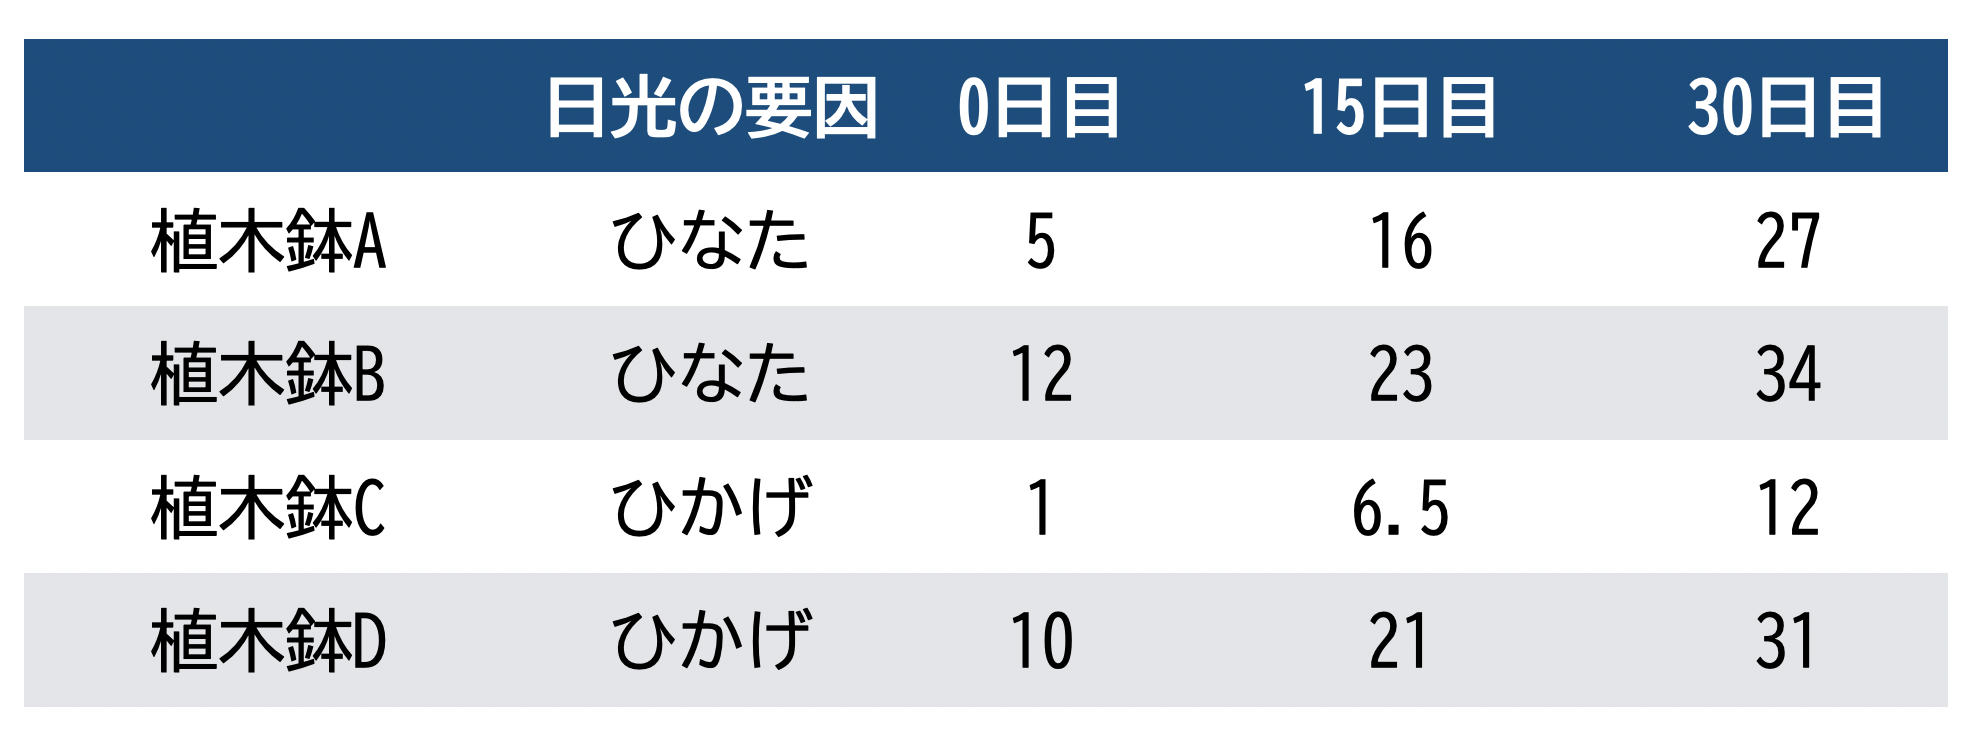
\includegraphics[keepaspectratio,width=0.8\linewidth]{figures/17_RCT/example_between.png}
\end{figure}


このときに考えられる要因の1つはもちろん日光ですが，これは1行目+2行目と3行目+4行目の条件を比較すればわかることになります。ただしこの実験はそれ以外にもたくさんの情報を含んでいます。それは1つの行が1つの植木鉢についての繰り返し獲得できた情報だということに起因します。データを見ると，植木鉢Aとか植木鉢Cはそもそも初日でほとんど芽が出ていませんでした。それに対して植木鉢Bと植木鉢Dは，初日ですでに10センチ以上の芽が出ていたことになります。こうした実験開始時の個体差というのは，今回の研究でどのように考えるべきでしょうか。今回の研究では日光がどれぐらい成長を促進するかということに興味があるのであって，そもそもの個体差は興味がなく，何なら実験にとって邪魔な情報ですらあります。

成長の促進の度合いは0日目と15日目との差分，15日目と30日目との差分でもって表されることであって，スタート地点の情報は必要ありません。 同じ鉢から反復してデータを得ているわけですから，行方向に数字を見ていくことによって，個体差を取り除いた変化量を考えることができます(図\ref{fig:17_03})。
\begin{figure}[ht]
	\centering
	\caption{比較できる方向}
	\label{fig:17_03}
	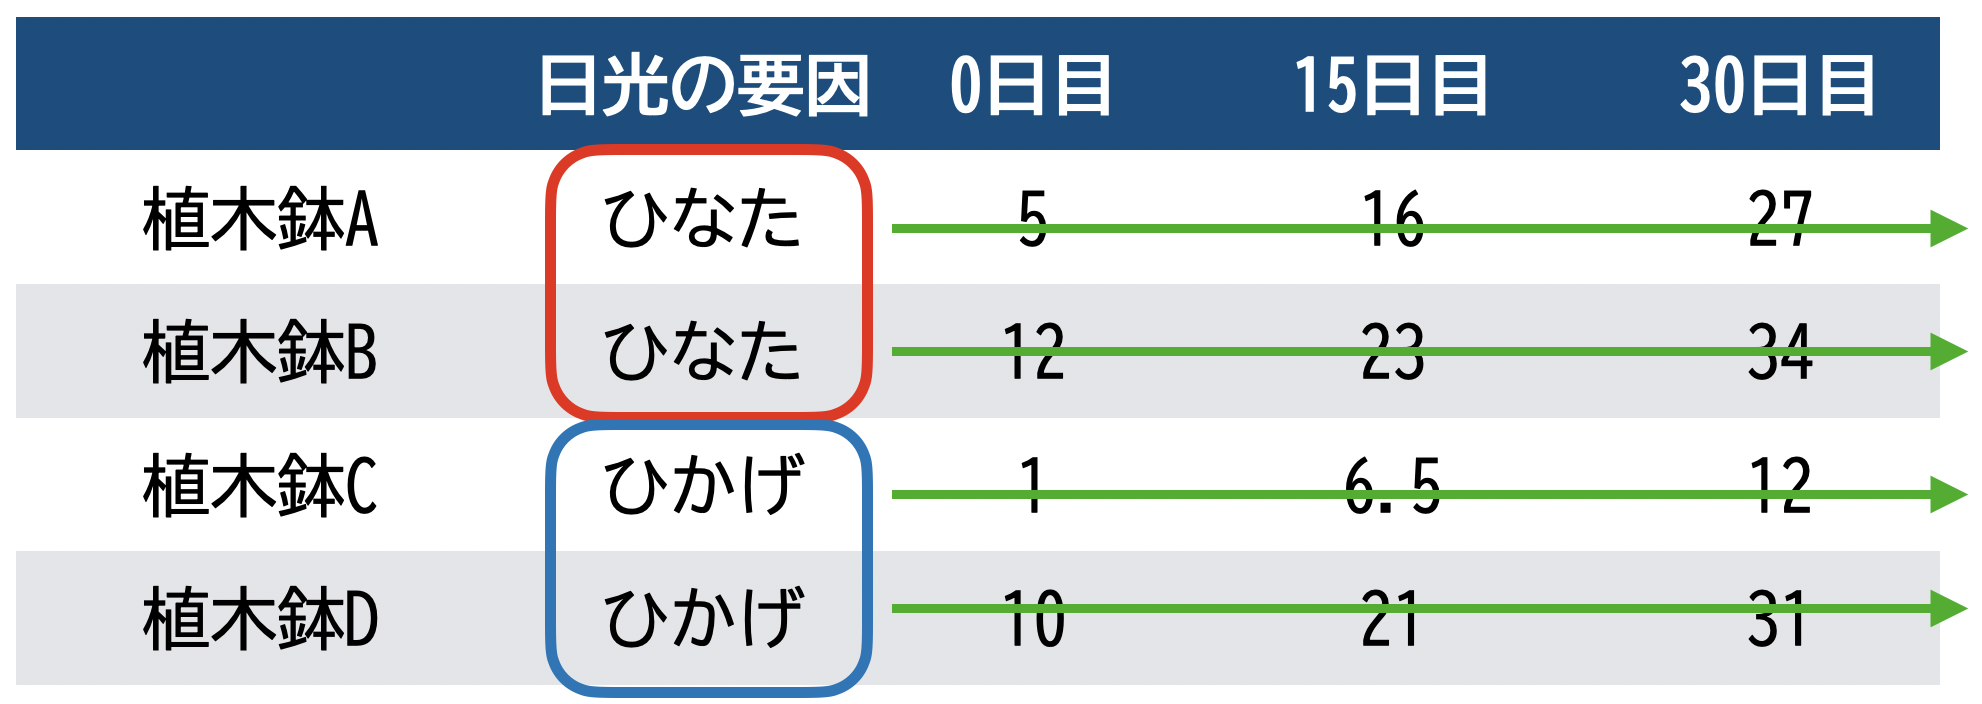
\includegraphics[keepaspectratio,width=0.8\linewidth]{figures/17_RCT/example_between2.png}
\end{figure}

このように，日向と日陰といったグループ間の違いを見る要因と，個体差を考慮して1つ1つの個体がどのように変化していったかを見るグループ内の違いを見る要因があります。用語としてそれぞれ\keyterm{群間要因}{ぐんかんよういん}{between factor}と\keyterm{群内要因}{ぐんないよういん}{within factor}といいます。今回の例では，日光を群間要因，測定日を群内要因と呼ぶことになります(図\ref{fig:17_04})。

この実験は群内要因と群間要因が組み合わさっていますので，とくに\keyterm{混合要因計画}{こんごうよういんけいかく}{mixed design}と呼ばれることもあります。水準数にも配慮して表現すれば，この研究は2要因の2$\times$ 3デザインあるいは「間2$\times$内3の混合計画」という言い方をします。
\begin{figure}[ht]
	\centering
	\caption{群内要因と群間要因}
	\label{fig:17_04}
	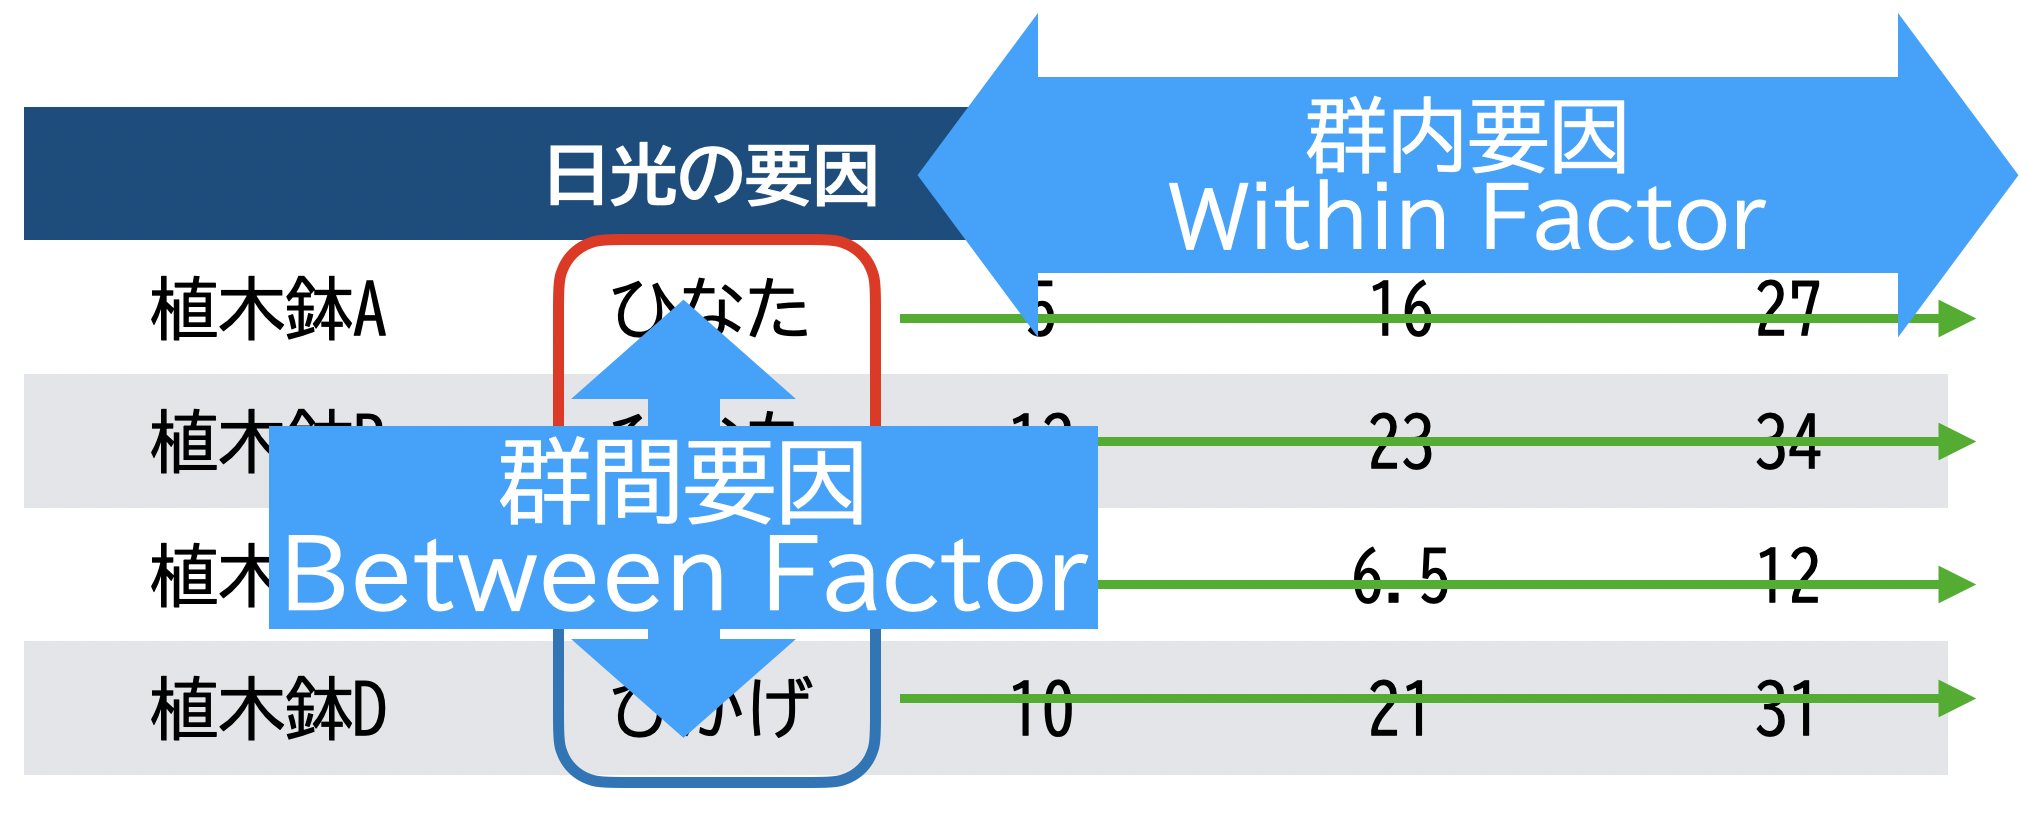
\includegraphics[keepaspectratio,width=0.8\linewidth]{figures/17_RCT/mixed_design.png}
\end{figure}

皆さんが実験を計画するときには，これらの言葉を使ってどういった要因を考え，どういった計画を立てているのかを表現する必要があります。ちなみに群間要因は別名\keytermLsub{対応のない}{たいおうのない}{群間要因}{ぐんかんよういん}要因とも言います。対して群内要因は，\keytermLsub{対応のある}{たいおうのある}{群内要因}{ぐんないよういん}要因，あるいはそのデータの性質から\keyterm{反復測定}{はんぷくそくてい}{repeated measure}要因とも呼ばれます。

後ほどの講義で詳しく説明されますが，群間要因計画と群内要因計画を比べると，群内要因計画の方が個人差を算出できることから，より精度の高い分析になります。群間要因計画は\keytermL{個人差}{こじんさ}と\keytermL{偶然誤差}{ぐうぜんごさ}を区別できないため，群内要因計画に比べると分析の精度は下がります。じゃあ全部群内要因で実験を計画すればいいじゃないかと思うかもしれませんが，群内要因の別名，「反復測定」という言葉にあるように，人を対象にする実験計画はそのまま実験参加者に対する負担になります。そういったことも考えると，内容によっては群間要因計画にせざるをえないということも少なくありません。

また，人間を研究対象にする場合は，考えるべき要因がたくさんあることも少なくありません。あの要因もこの要因も関係してくるに違いないと考えると，実験計画の要因数はどんどん増えていきます。ただしこの後見ていくように，要因をどんどん増やすと組み合わせを考慮しなければならない数も多くなり，解釈も難しくなりますから，せいぜい3要因で，できれば2要因までで研究計画をすることをお勧めします。

\section{効果はどのように評価するのか}
\label{HowToEvaluateTheDifference}

\begin{figure}[ht]
	\centering
	\caption{平均値の差(群の効果)が同じ2つの実験の例。どちらの実験が効果があると言いやすいか。}
	\label{fig:17_05}
	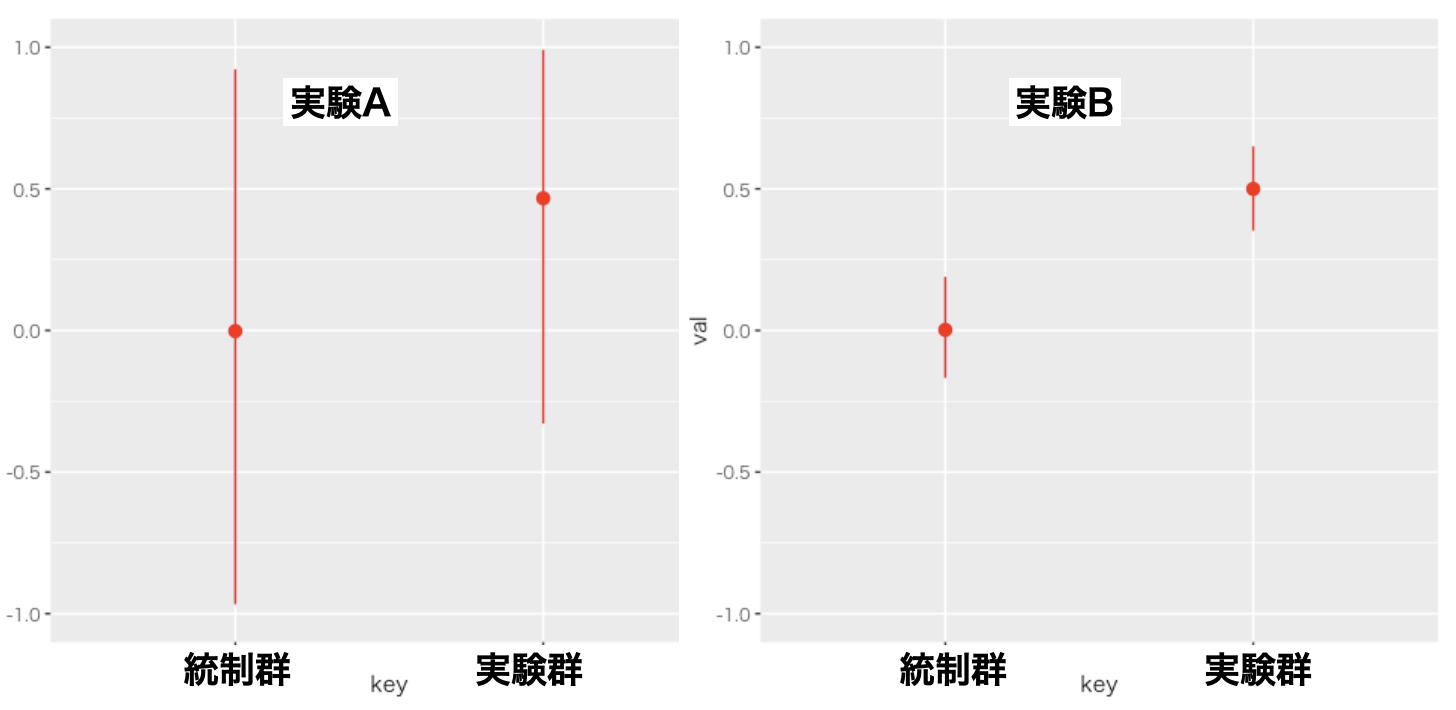
\includegraphics[keepaspectratio,width=0.8\linewidth]{figures/17_RCT/effectSize.png}
\end{figure}

ここで図\ref{fig:17_05}を見てください。左に実験A，右に実験Bとふたつの実験結果を示しています。これは箱ひげ図の箱をとったような図で，赤い点が群の平均値，そこから上下に伸びる線は群の最大値と最小値を結んでいます。
実験Aは実験Bに比べて，分散が大きいのがすぐにわかると思います。実は実験Aと実験Bは，平均値間の差は同じです。この時，実験の効果があった，とはっきり言い切れるのはどちらでしょうか？

実験Aの方は，確かに実験群のほうが平均値が高くなっていますが，統制群の中にいる最大値の人は実験群の中の数字と遜色ないですし，実験群の最小値の人は統制群に入っててもおかしくない数字です。
これに対して実験Bの方は，統制群の最大値でも実験群の最小値におよびません。いくら頑張っても実験群ほどのスコアを出せないのですから，これは実験群による介入の効果が大きかったと判断しやすくなりますね。

つまり実験によって効果があった，なかったという評価をする時は，\textbf{群内の分散に比べて群間の分散が十分大きいかどうか}で考えることになります(図\ref{fig:17_06})。
\begin{figure}[ht]
	\centering
	\caption{平均値の差(群の効果)が同じ2つの実験の例。左側は群間の分散(緑の矢印)に比べて群内の分散(青の矢印)が大きいため，効果があるとは言いにくい。右側の例では，統制群の最大値が実験群の最小値にも及ばないほどなので，効果があると言いやすい。}
	\label{fig:17_06}
	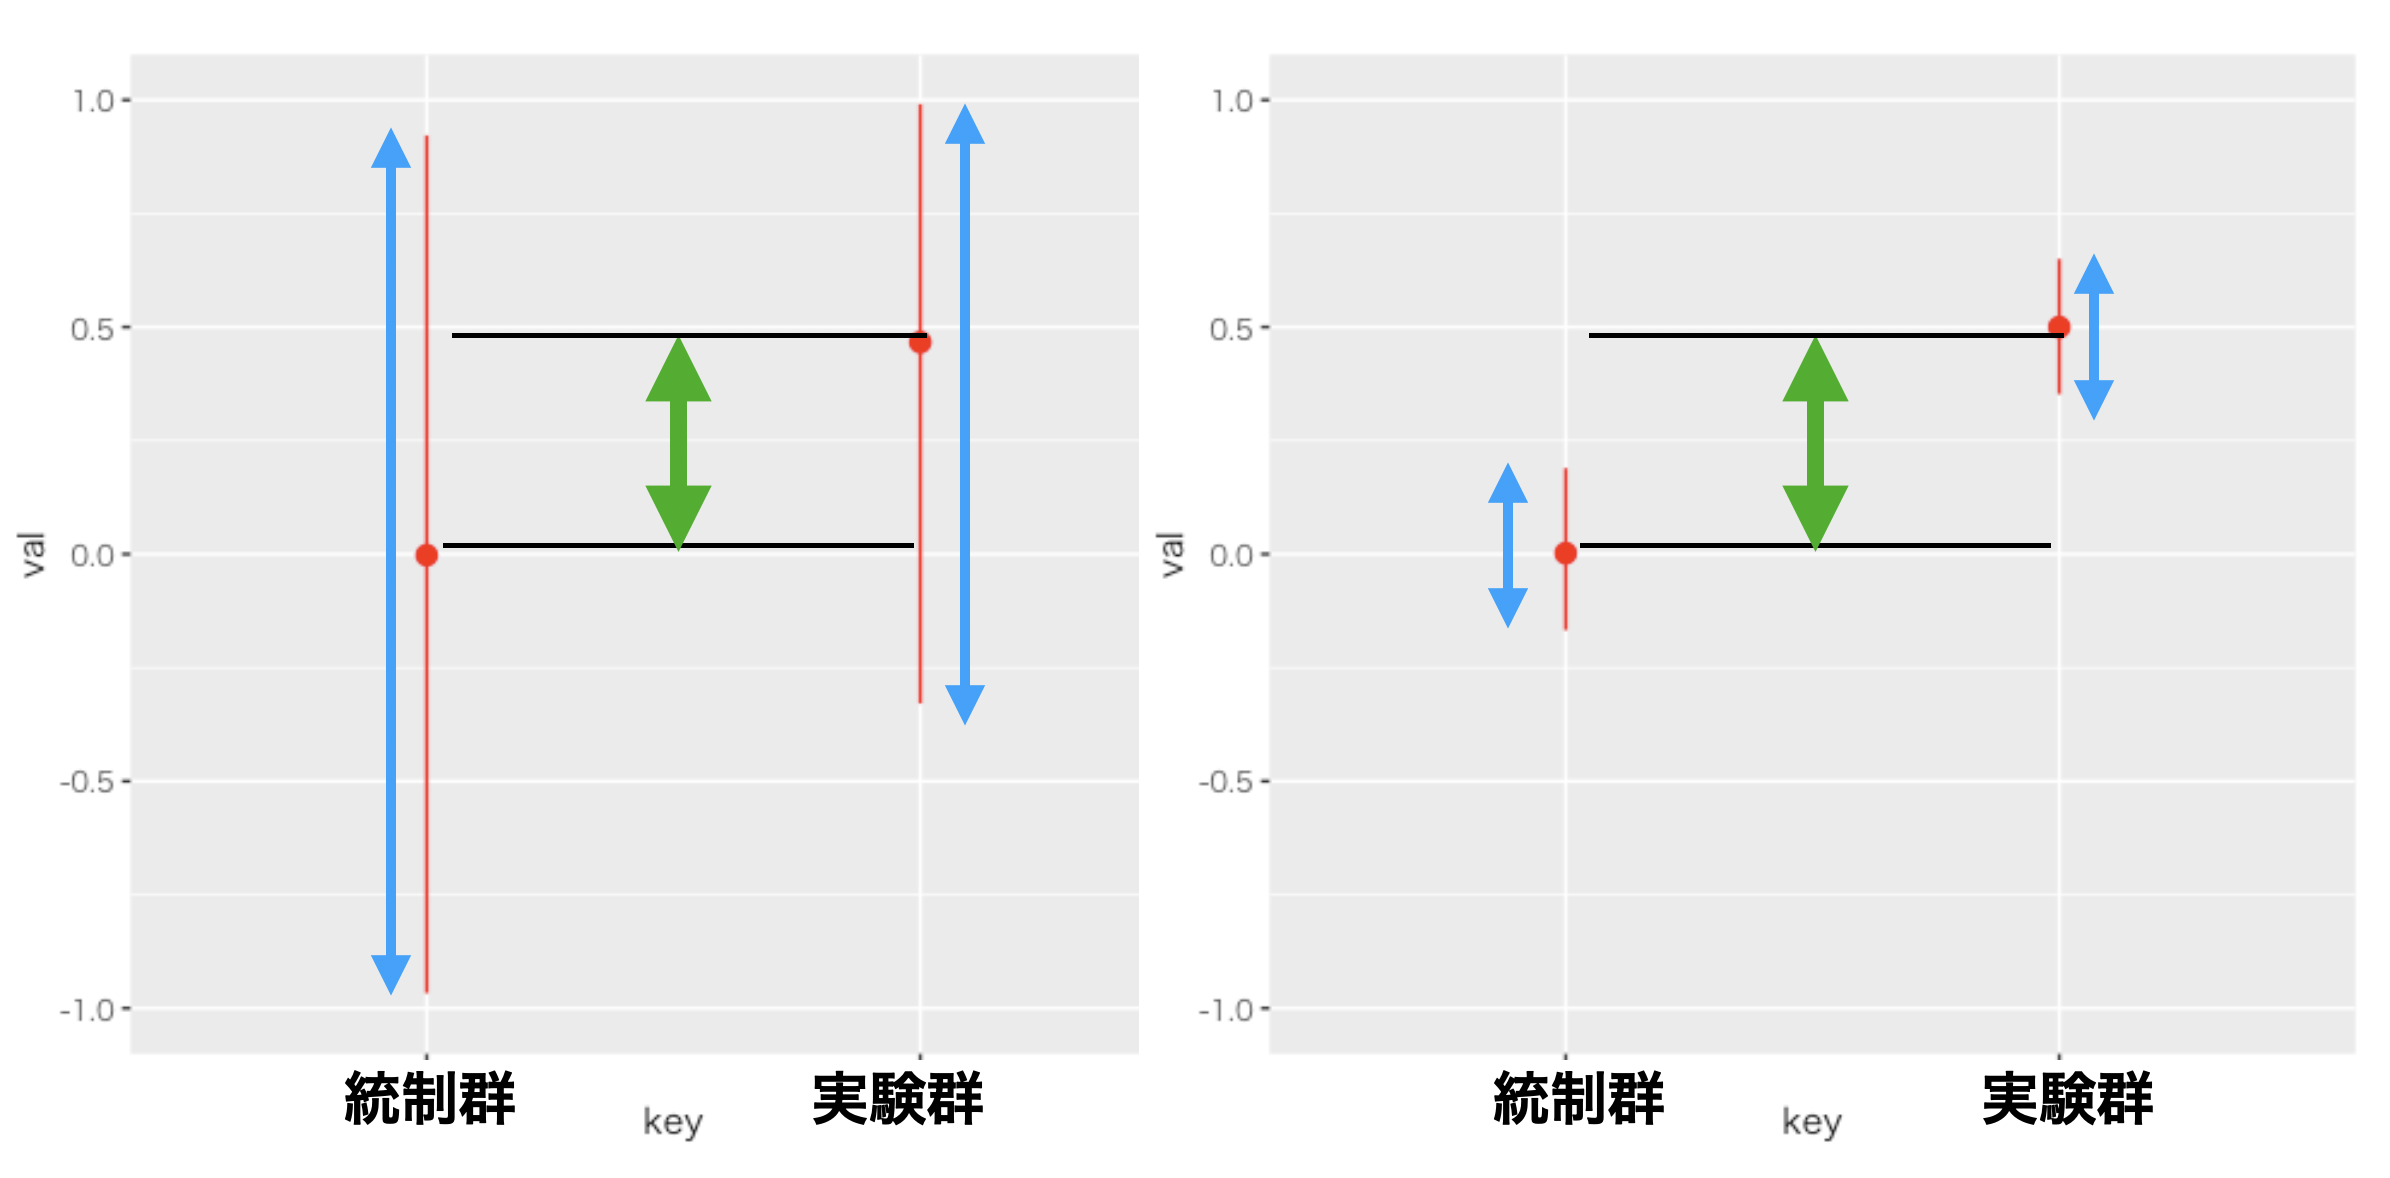
\includegraphics[keepaspectratio,width=0.8\linewidth]{figures/17_RCT/effectSize2.png}
\end{figure}

何らかの効果を評価するときに，誤差に比べた大きさで考えるというのは重要なポイントです。統計的な有意差は「帰無仮説が正しい」とした世界での(仮想空間での)判断基準に過ぎず，実際にはどれぐらい意味のある効果だったのか，ということが大事だという話はすでにした通りです。有意差でなく，実際の差。あるいは，標準化された差で考えることが重要です。標準化された差のことを\keyterm{効果量}{こうかりょう}{effect size}というのでした。この効果量，特に平均値差の効果量は，群間の分散に比べて群内の分散がどれぐらい小さいか，ということを数値化したものです。群間(要因の水準間)の分散が大きく，群内(要因の操作では測れない変動)の分散が小さいほど，効果量は大きくなります。この効果量が大事であるということと，多水準間での比較の話は，軌を一にするものなのです。


\section{線形モデルとしてみた要因計画}

要因計画に沿って得られたデータにおいて，効果の大きさは誤差に対する比で検証することが重要だ，という話でしたが，これを少し具体的な計算モデルで考えてみましょう。そう，平均値の差を比べるというのも，統計的なモデルに基づいた計算になるのです。ここまでの話でどこに「モデル」の話があったのか？と思う人がいるかもしれません。あるいは，また新しいモデル(数式)の話か，と思う人もいるかもしれませんが，大丈夫，実は皆さん既に学んだモデルの話なのです。ここからは，「要因計画は回帰分析と同じ線形モデルだったのだ」という話をしていきます。

さて，帰無仮説検定の話をしたときに，これはモデル比較だと言いました($\to$セクション\ref{sec:13_02}，Pp.\pageref{sec:13_02})。帰無仮説というモデル，対立仮説というモデルを比較して，どちらに軍配を上げるかという勝負判定をする，これが帰無仮説検定だと。

ここでの「モデル」という言葉は，データがどのように作られているかを数式で記述したもの，という意味です。実は巧妙に隠されているんです。
前回の2群の平均値差の話を思い出してください。要因計画の文脈で言えば，2群の平均値差の検定は，「一要因二水準計画」です。対応のある検定は群内計画，対応のないものは群間計画です。

ここでは例として，群間の一要因二水準計画で考えてみましょう。
実験群と統制群のデータが得られたとしましょう，という話から始まりましたね。それぞれの群に含まれる個体の背景には様々な影響があって，個人差もいっぱいありますし，偶然誤差も含まれます。そこで得られたデータが正規分布に従う，と仮定してみましょう。実験群も統制群も，同じ正規分布($N(\mu,\sigma)$)から得られたデータです。

片方の実験群には何らかの心理学的な介入をして，もう片方の統制群には何もしません。とすると，統制群の方は実験前の平均値と分散に変化がなく(何もしていないのですから)，$N(\mu,\sigma)$のままです。実験群の方は，心理学的な介入をしたので，平均値が変化して$N(\mu+\delta,\sigma)$となったとします。ここで$\delta$は介入の効果です。

\begin{figure}[ht]
	\centering
	\caption{再掲；対応のない二群の平均値差の検定のシーン}
	\label{fig:17_07}
	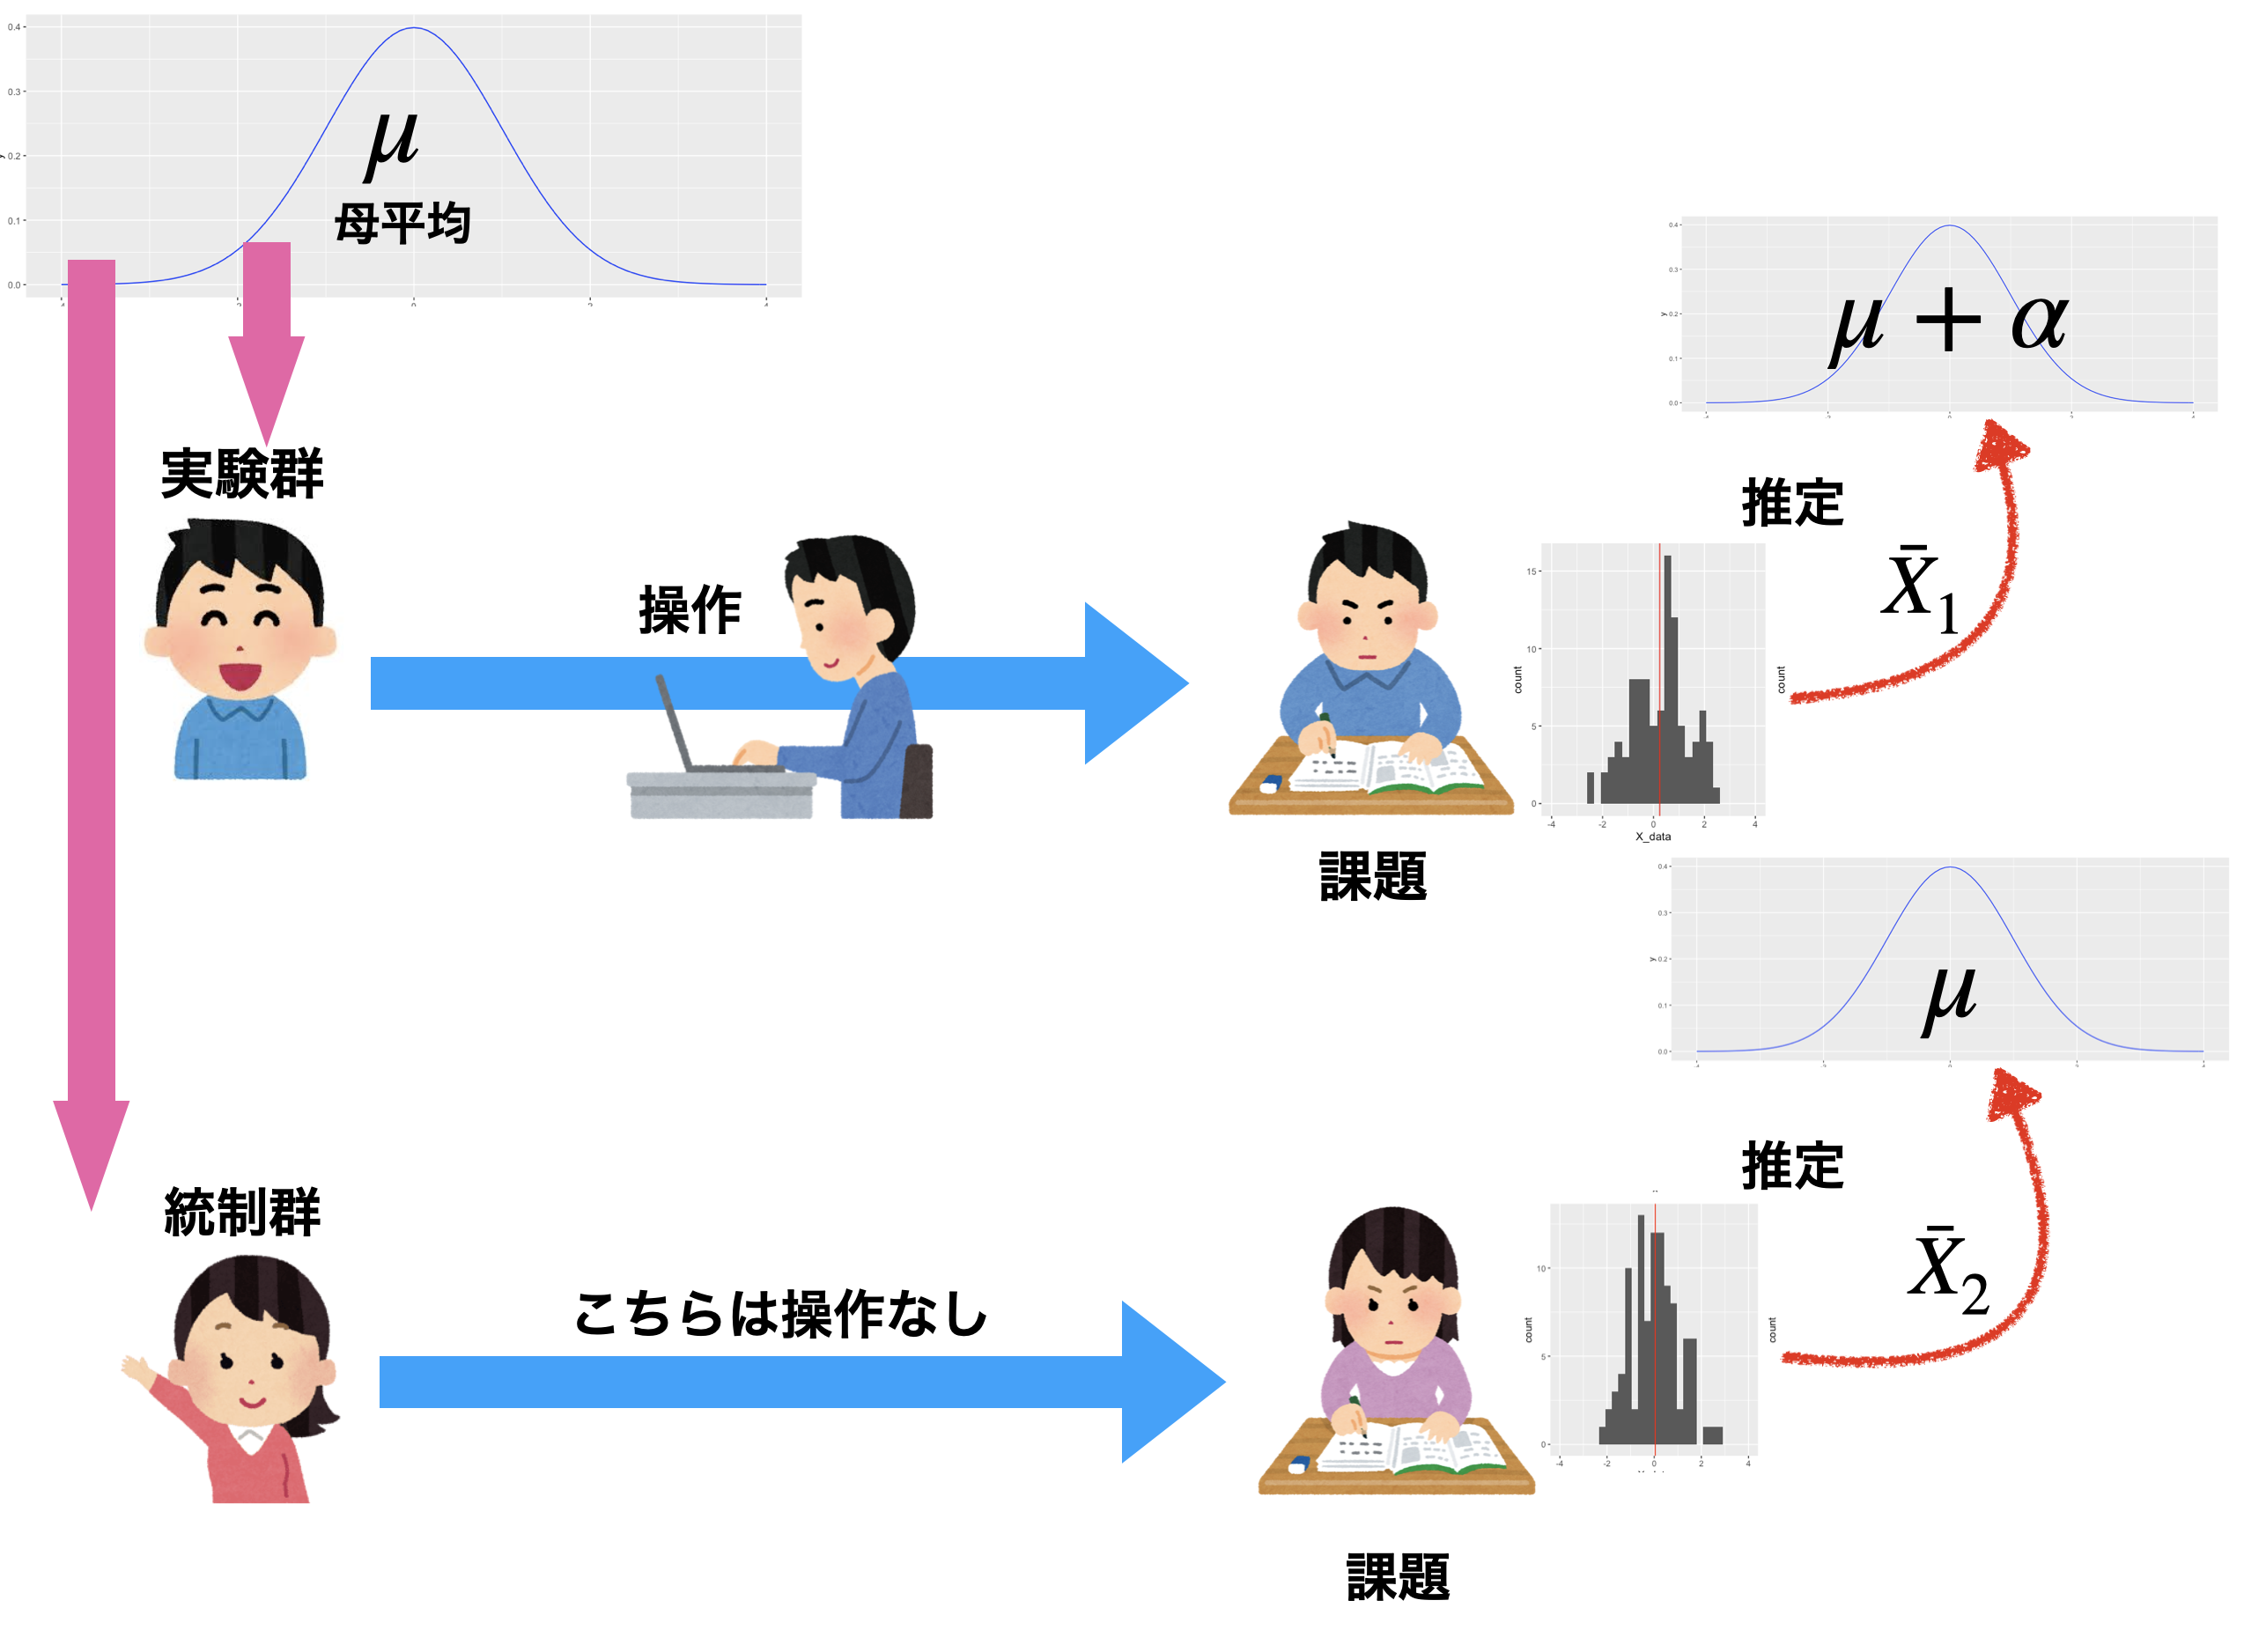
\includegraphics[keepaspectratio,width=0.8\linewidth]{figures/16_ttest/independent_t.png}
\end{figure}

はいこれ！これがモデルです！
え，どこが，と思うかもしれません。モデルは「データがどのように作られているかを記述したもの」でしたね。ここでのモデルは，「データが正規分布によって生み出されている」ということ，そのものなのです。カッコつけて書くと，

\begin{align}
X_A \sim N(\mu,\sigma),\quad X_B \sim N(\mu+\delta,\sigma)
\end{align}

と書くことができます。ここで$X_A$は統制群のデータ，$X_B$は実験群のデータです。データがどうやって作られたか，数式で書かれているでしょう！

そして検定の時は「帰無仮説モデル」vs「対立仮説モデル」とするのでした。帰無仮説モデルは母平均に差がないというモデルですから，$\delta=0$というのがそれです。対立仮説モデルは$\delta \neq 0$です。

具体的に考える例として，次のようなデータを用意しました(図\ref{fig:17_08})。これは対応のない，2つの群(仮に実験群と統制群とします)の平均値をプロットしたものです。ここで示されている平均値は標本平均ですから，そこに差があるのは見た通りです。ちなみに黒い点は各群における個体1つ1つの観測値です。

\begin{figure}[ht]
	\centering
	\caption{2つの群の平均値のプロット。黒い点は各群のそれぞれの観測値}
	\label{fig:17_08}
	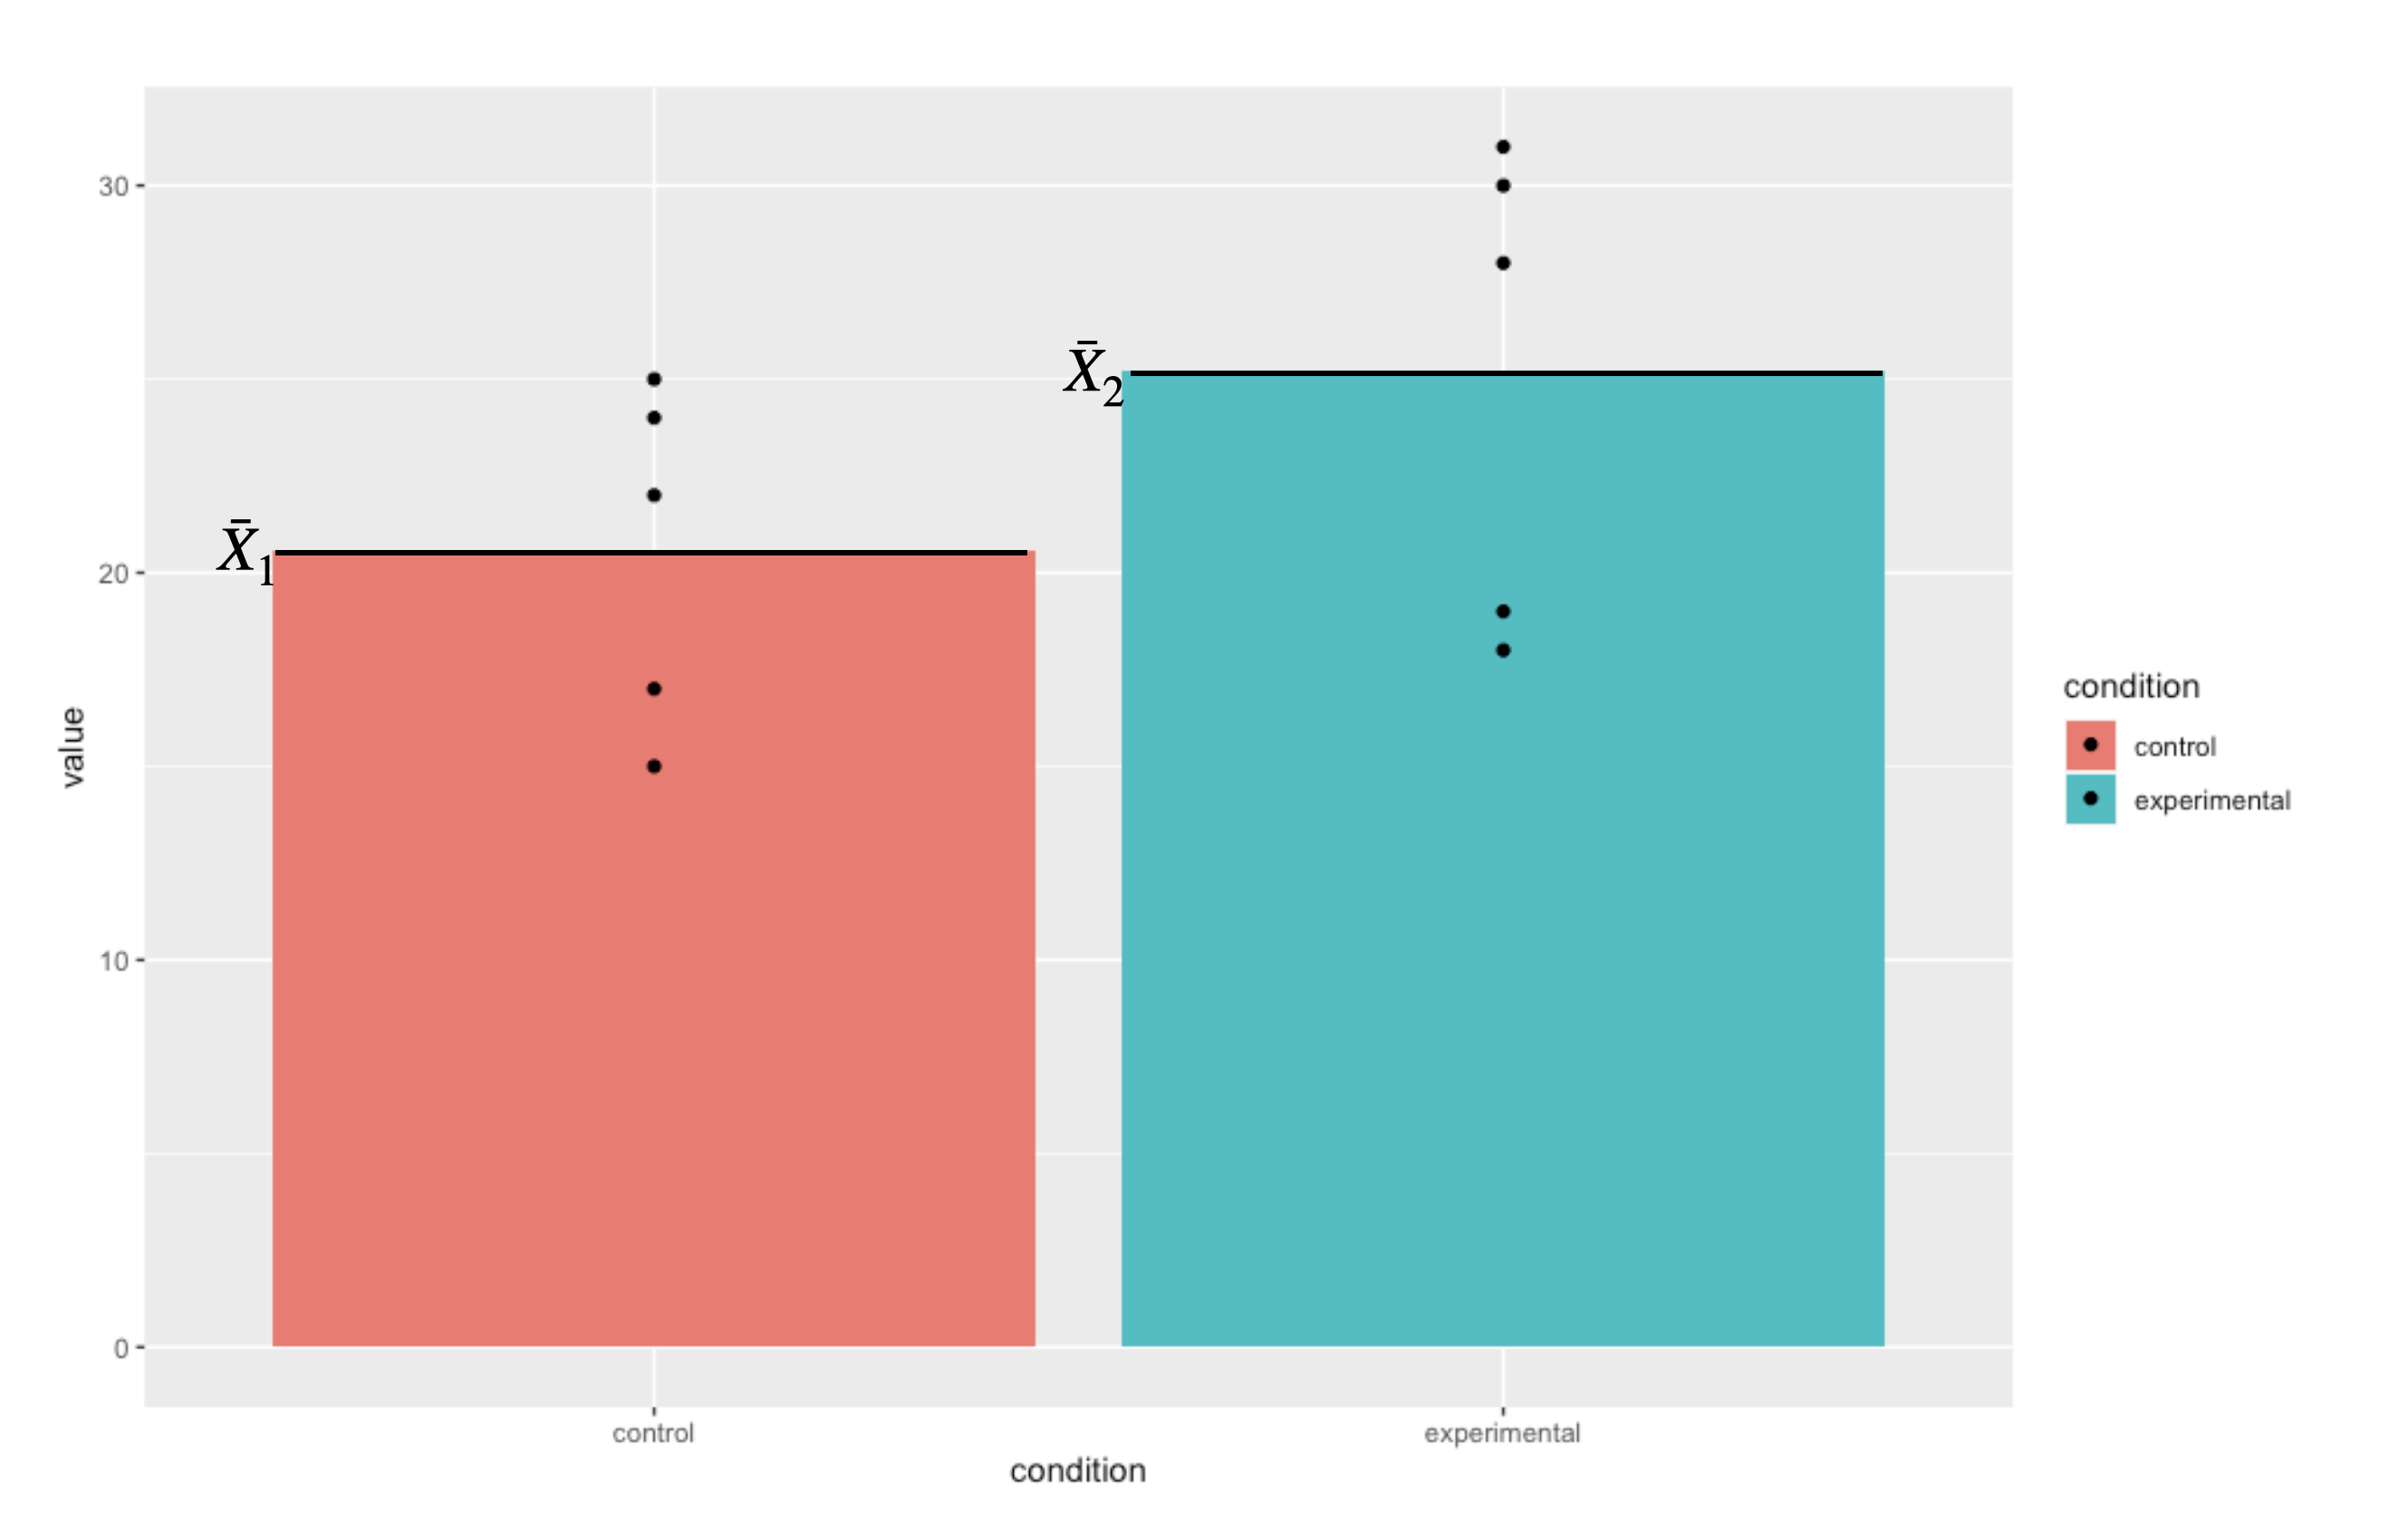
\includegraphics[keepaspectratio,width=0.75\linewidth]{figures/19_Ftest/two_levels.png}
\end{figure}

今回の例において，従属変数である心理変数はどういう特徴なのか，目に見えないものなのでわかりません。でも，心の問題は無数の要因が積み重なった結果であると考えると，正規分布を仮定するのが自然です。つまり，実験群のひとも統制群のひとも，大きな視点から考えれば同じ人間という正規母集団からのサンプルなのです。

さて，実験参加者たちは実験者によって無作為に実験群と統制群に割り当てられました(RCT)。個人差がなければ，各群1名ずつのスコアを比較して考えれば良いのですが，人間を対象にしている以上そうはいきません。個人差がどうしても生じてしまうので，複数人を集めて個人差を相殺することを考えます。各群の平均値の違いを見ることで，操作の効果を見ることにするのです。

もしこの実験に効果がなければ，2群の平均値は同じになるでしょう。この時の平均値は，実験群と統制群に分けた効果がないのですから，両群のスコアを足しあわせた全体平均になるはずです。効果がない=全体平均，なのです。しかし，群ごとに見てみると全体平均から違いが生じています。図\ref{fig:17_09}では，統制群は相対的に低く，実験群は相対的に高い平均値を示しています。この差分こそ(図\ref{fig:17_09}では短い緑の矢印で示しています)，実験の効果なのです。

\begin{figure}[hb]
	\centering
	\caption{効果がなければ全体平均に同じ。群の効果は相対的に平均値をずらす。}
	\label{fig:17_09}
	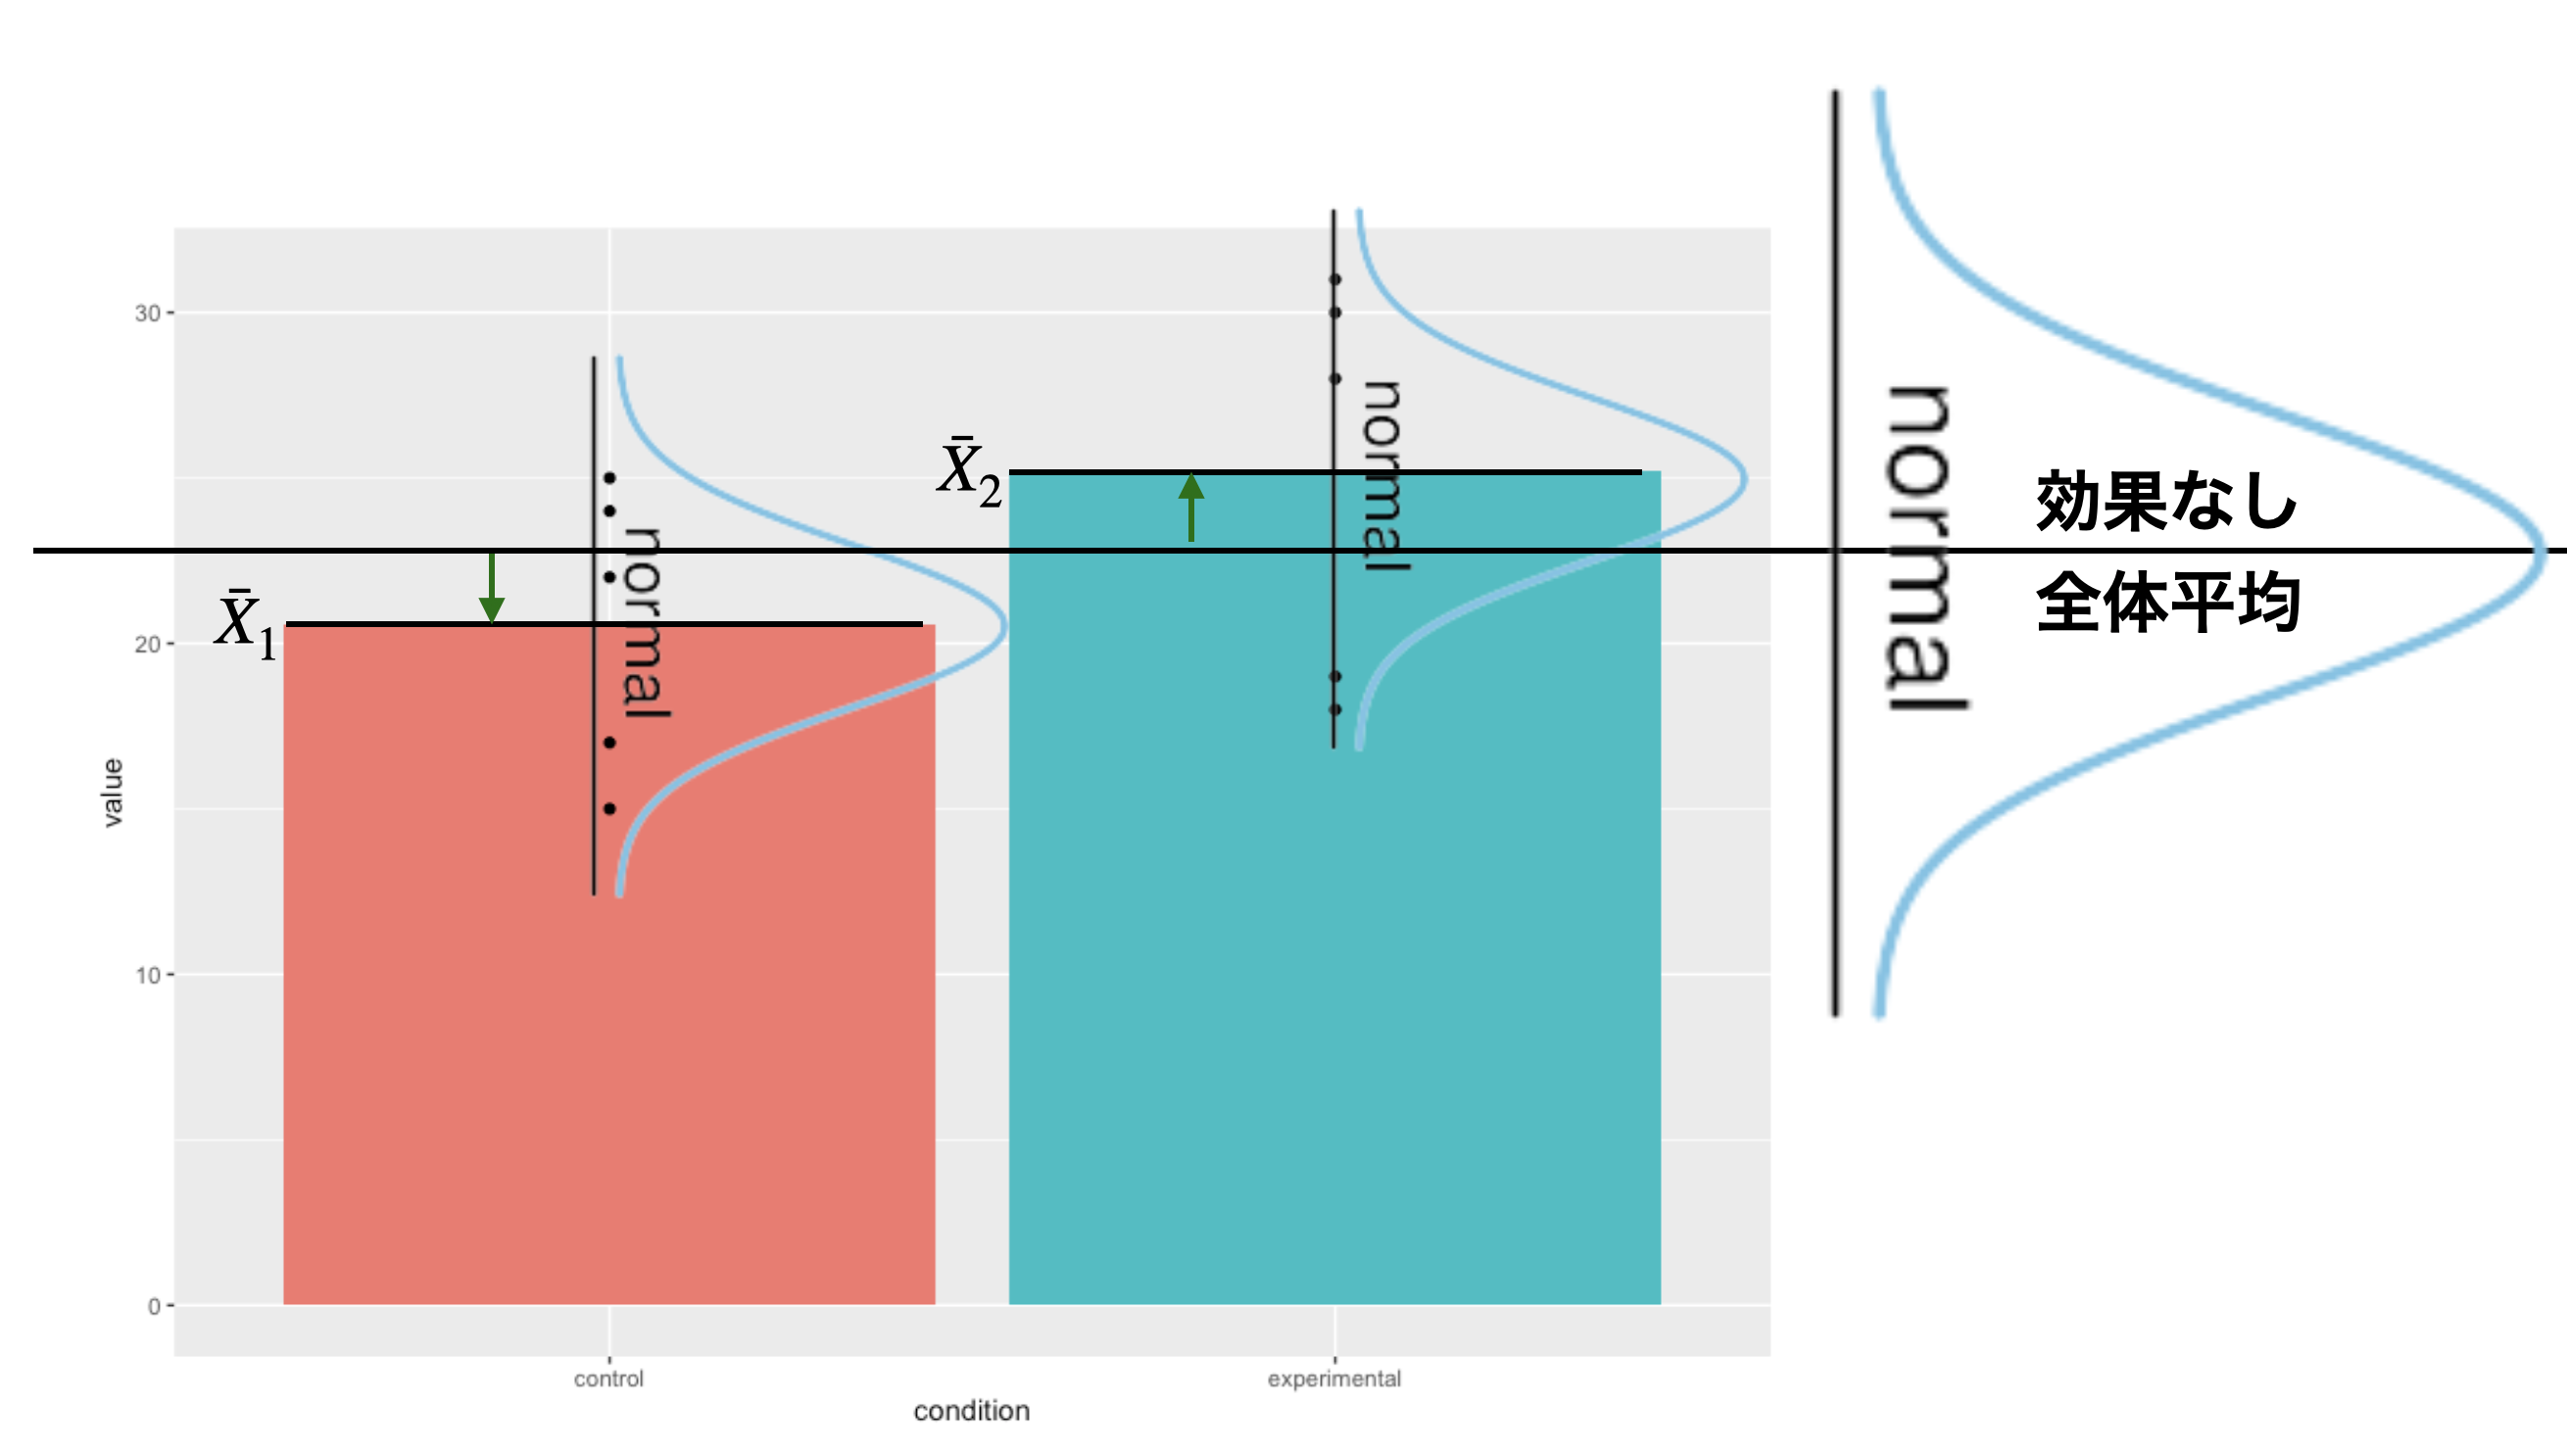
\includegraphics[keepaspectratio,width=0.8\linewidth]{figures/19_Ftest/two_levels_norm.png}
\end{figure}

さて，群ごとの平均は次のように書くことができます。
\begin{align}
\bar{X}_1 =\frac{1}{5} \sum_{i=1}^5 X_{i1}
\end{align}
\begin{align}
\bar{X}_2 =\frac{1}{5} \sum_{i=1}^5 X_{i2}
\end{align}
また，全体平均は次のように書くことができます\footnote{gmはgrand meanの略です。}。
\begin{align}
\bar{X}_{gm} = \frac{1}{10} \sum_{i} \sum_{j} X_{ij}
\end{align}
これは標本を使った平均値ですが，本来は推定したい(群間の差がない)母平均について議論したいところです。$\bar{X}_{gm}$は母平均の推定値として使い道はありますが，理想化・抽象化して語れるのがモデルの良いところですから，ここでは全体平均を未知数を表すギリシア文字$\beta$をつかって$\beta_0$としておきましょう。

さて次に，群わけの効果を$\beta_1$としましょう。すると各群の平均のモデルは
\begin{align}
\mu_1= \beta_0 + \beta_1
\end{align}
\begin{align}
\mu_2 = \beta_0  -\beta_1
\end{align}
と表すことができます。左辺も各群の母平均なので，未知数を表すギリシア文字になっています。

つづいて，ここでの個人差はこの実験で制御できない誤差であり，群平均を中心にどういう向きで出るかわからないものですから，このことを表現するなら，
\begin{align}
X_{ij} = \mu_j + \varepsilon_{ij}
\end{align}
ということになります。これらを組み合わせると，
\begin{align}
X_{i1} = \beta_0 + \beta_1 + \varepsilon_{i1}
\end{align}
\begin{align}
X_{i2} = \beta_0 - \beta_1 + \varepsilon_{i2}
\end{align}
と書くことができます。ここで一工夫。$\beta_1$にプラス，マイナスの符号がついているのは，$+1,-1$を掛け算していると考えてみましょう。この符号を決めているものを$X_{1}=+1,X_{2}=-1$と表したとすると，まとめて次のように書くことができます。
\begin{equation}
	\label{eq:19_01}
	X_{ij} = \beta_0 +  \beta_1 X_{j} + \varepsilon_{ij}
\end{equation}


Oh La La!どこかで見たことありませんか，この式の形？\footnote{Oh La La!はフランス語で「おやまあ！」という意味ですが，筆者は映画Back to the Future Part 2に出てきたセリフとして知っています。}


そう，\keytermL{線形モデル}{せんけいもでる}ですね！$y_i=b_0 + b_1x_i + e_i$と同じ，すなわち個々の値($y_i$)が，全体平均($b_0$)と効果($b_1x_i$)と誤差($e_i$)に分解されています。\textbf{実験計画は線形モデルだったのです。}\label{experiment_is_lm}
違いは$x_i$が説明変数の大きさではなくて，どの群に含まれているかを表す離散的な変数になっているということだけです。回帰分析では独立変数も従属変数も連続変数だったのですが，説明変数が離散的な回帰分析のことを我々は実験(計画)と呼んでいるのです。

要因計画の式\ref{eq:19_01}において，$X_j$はダミー変数と呼ばれるもので，2つの群を区別するために使われています。$j=1$ならば$X_j=+1$，$j=2$ならば$X_j=-1$となります。

1つの共通の正規分布。2つの群に分かれない，同じ正規分布。そろそろ帰無仮説検定と繋がってきたのではないでしょうか。効果がない，というのはまさに，帰無仮説のことですよね。つまり帰無仮説は，$\beta_1=0$という傾きゼロの直線，図\ref{fig:17_09}では群平均を横切っている，横一線の線形モデルだったのです。平均値の差の検定というのは，群平均が横一直線＝傾きゼロではないよ，という結論を出すためのロジックであり，比較される対立仮説は「傾きゼロでない何か」というモデルです。
\begin{itemize}
	\item 帰無仮説H0: $\mu_1 = \mu_2$ $\to$ 線形モデルにおける傾きの係数$\beta_1=0$
	\item 対立仮説H1: $\mu_1 \neq \mu_2$ $\to$ 線形モデルにおける傾きの係数$\beta_1\neq 0$
\end{itemize}
帰無仮説が傾きゼロという一点ばりに対し，対立仮説はゼロ以外であれば何でも良いというラフなモデルです。ですから帰無仮説が棄却されたとしても「差がなくはない」という程度のもので，「じゃあゼロでない，何なのか」ということまでは強く主張できません。何度も繰り返すようですが，実質はどのように傾いているのか，差の信頼区間はどの程度あるのか，効果量(標準化された平均値の差)は大きいのかといった，実質的な大きさを考えることが重要だ，ということを忘れないでください。


\section{課題}
\paragraph{要因と水準}次の心理学実験は，どのような要因計画でできているでしょうか。要因，水準という言葉の違いに注意しながら，正しく表現してみましょう。

例)「3つの学校で共通試験をした。成績の平均値に差があるかどうかを検証したい。」$\to$ 一要因3水準，群間(Between)デザイン

\begin{itemize}
	\item アサガオの生長を観察するため，水をあげる群とあげない群，肥料をあげる群とあげない群をつくり，成長の程度を比較した。
	\item ラットの種類A/Bそれぞれに対して，トランキライザーの効果を見るため，0.4mg/0.7mg/1.5mg投与する群を作り比較した。
	\item 4つの学校で，1年間で共通の試験を実施した。一学期，二学期，三学期の各校における成績変化を比較したい。
	\item 二つの社会的強化の方法(a1,a2)があり，この条件に無作為に大学生を選び割り当てた。被験者は4つのセッション(b1,b2,b3,b4)を体験し，各セッションの作業量を調べ，比較する。
\end{itemize}


\end{document}
